\documentclass{../../slides-style}

\slidetitle{Практика: Множество на основе хеш-таблицы}{26.09.2026}

\begin{document}

    \begin{frame}[plain]
        \titlepage
    \end{frame}

    \section{Введение, хеш-таблица на списках}

    \begin{frame}{Напоминание про хеш-таблицы}
        \begin{outline}
            \1 Вероятностная структура данных, основа для реализации множеств и словарей
            \1 Позволяет достичь \enquote{почти} константного времени выполнения базовых операций (вставки, удаления, проверки на принадлежность/поиска) при довольно небольших накладных расходах
                \2 ведёт себя как массив, где индексами могут быть значения произвольного типа
            \1 Хранят значения \enquote{перемешанными}
            \1 Реализуются на массивах (т.н. \enquote{открытая адресация}) и на списках
                \2 на массивах работает побыстрее, но в образовательном смысле на списках нам интереснее
        \end{outline}
    \end{frame}

    \begin{frame}{Хеш-функции}
        \begin{outline}
            \1 Некоторая функция, отображающая большое (потенциально бесконечное) множество ключей в конечное (и маленькое) множество хеш-значений
            \1 Чем \enquote{случайнее} она это делает, тем лучше
            \1 Зачем: факторизуем множество ключей по классам эквивалентности, образованным ключами с равными хеш-значениями, будем хранить в массиве фактор-множества
                \2 чем лучше хеш-функция, тем равномернее значения будут раскладываться по хеш-таблице
        \end{outline}
        \begin{center}
            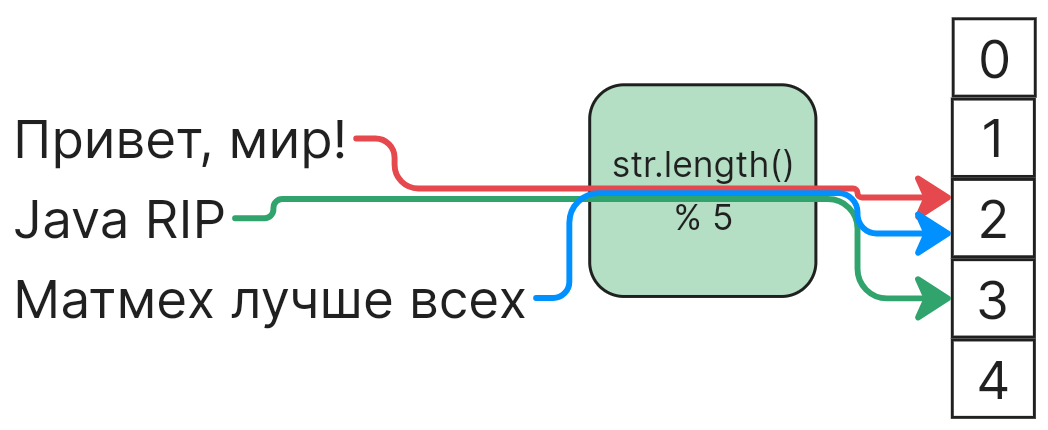
\includegraphics[width=0.7\textwidth]{hashFunction.png}
        \end{center}
    \end{frame}

    \begin{frame}{Хеш-таблицы на списках}
        \begin{outline}
            \1 Заведём массив с числом элементов, примерно равным ожидаемому размеру множества
            \1 Сделаем хеш-функцию, множество значений которой --- индексы массива
                \2 проще всего --- взять хеш-функцию, которая просто считает неотрицательное целое, и брать остаток от деления на длину массива
            \1 В каждой ячейке массива --- список из значений
            \1 Если у двух элементов хеш-значения совпадают, просто кладём их в список подряд
        \end{outline}
        \begin{center}
            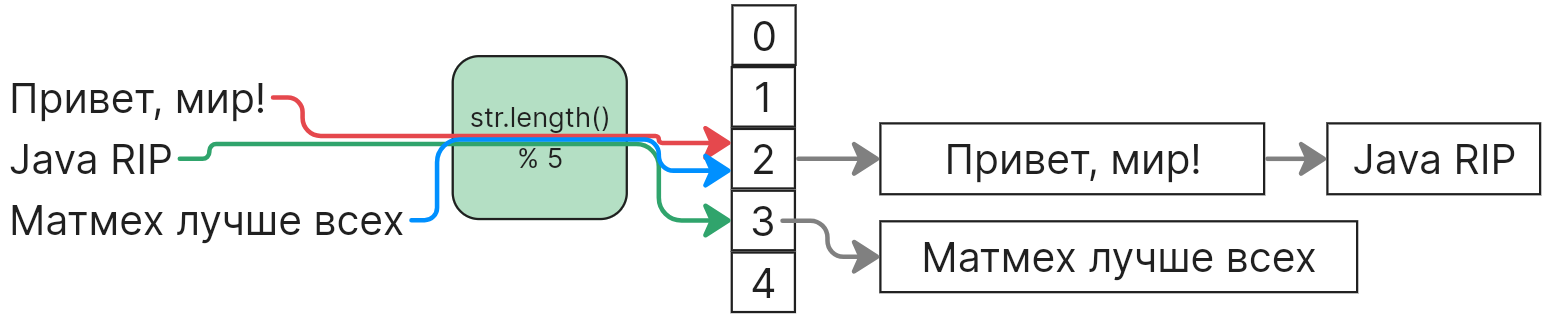
\includegraphics[width=0.7\textwidth]{hashTable.png}
        \end{center}
    \end{frame}

    \begin{frame}{Базовые операции}
        \begin{outline}
            \1 Добавление: считаем хеш-функцию, находим индекс в массиве, добавляем в голову списка
                \2 $O(1)$
            \1 Удаление: считаем хеш-функцию, находим индекс в массиве, бежим по списку, сравниваем, если нашли --- удаляем из списка
                \2 $O($длина списка$)$
            \1 Поиск: считаем хеш-функцию, находим индекс в массиве, бежим по списку, сравниваем, если не нашли --- элемента нет
                \2 $O($длина списка$)$
        \end{outline}
        \begin{center}
            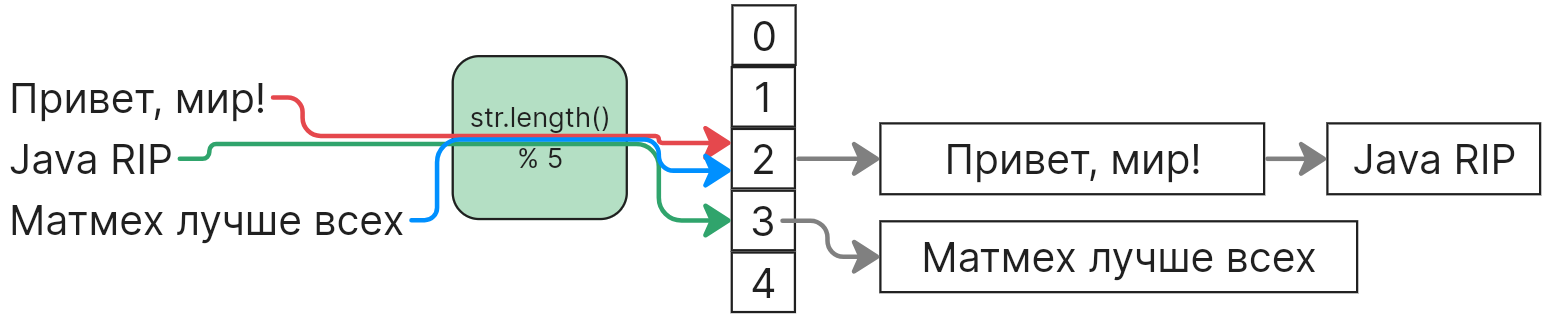
\includegraphics[width=0.7\textwidth]{hashTable.png}
        \end{center}
    \end{frame}

    \begin{frame}{Тонкости}
        \begin{outline}
            \1 Если хеш-функция хорошая, длина списка обычно равна количеству элементов множества, делённому на количество ячеек в массиве
                \2 это называется \enquote{коэффициент заполнения} (load factor)
                \2 в идеале для хеш-таблиц на списках коэффициент заполнения должен быть равен 1
                    \3 тогда базовые операции имеют константную трудоёмкость
                    \3 слишком низкий коэффициент заполнения --- лишние расходы памяти
            \1 Количество хранимых данных, как правило, заранее неизвестно, поэтому хеш-таблица динамически меняет размер
                \2 при каждом добавлении проверяем коэффициент заполнения, если он больше 1, увеличиваем массив вдвое
                \2 размер массива участвует в хеш-функции, так что все элементы надо переложить
                    \3 иначе их потом не найти будет
        \end{outline}
    \end{frame}

    \begin{frame}{Выбор хеш-функции}
        \begin{outline}
            \1 Пример достаточно хорошей хеш-функции для строки: $a[0]*p^n + a[1]*p^{n - 1} + … + a[n]$, особенно если $p$ --- простое (Rolling hash)
                \2 Считается в цикле \enquote{умножили предыдущее значение на $p$ и прибавили следующую букву}
            \1 Для чисел часто используется тождественная функция
            \1 Есть \mintinline{java}|Object.hashCode()|, переопределяемый для конкретных классов
                \2 как раз тождественная функция для чисел
                \2 по умолчанию значение указателя для ссылочных типов
                \2 возвращает произвольное целое (может быть отрицательным), его надо самим приводить в нужный диапазон
            \1 Бывают ещё криптографические хеш-функции (MD5, SHA-1, SHA-3, \dots), они долго считаются
            \1 Бывает идеальный хеш --- инъективная функция (т.е. не допускает коллизий)
        \end{outline}
    \end{frame}

    \section{Задача}

    \begin{frame}[fragile]{Задача}
        \begin{outline}
            \1 Поделиться на команды по 2-3 человека
            \1 Реализовать класс StringSet --- реализацию АТД \enquote{Множество} для строк на хеш-таблицах
            \1 Должны поддерживаться операции:
                \2 \mintinline{java}|void put(String element)| --- добавить элемент в множество
                \2 \mintinline{java}|bool remove(String element)| --- удалить элемент из множества 
                    \3 возвращает true, если операция завершилась успешно
                \2 \mintinline{java}|boolean contains(String element)| --- true, если данная строка принадлежит множеству
                \2 \mintinline{java}|int size()| --- количество элементов множества
                \2 \mintinline{java}|void clear()| --- очистить множество
        \end{outline}
    \end{frame}

    \begin{frame}[fragile]{Задача, ещё требования}
        \begin{outline}
            \1 Для реализации потребуется список, он должен быть реализован как отдельный класс
                \2 это должен быть связный список, на ссылках
                \2 достаточно только тех операций, которые нужны в данной задаче
            \1 Нужен код в main, который проверяет, что всё работает
                \2 но не увлекайтесь, на следующем занятии будем писать тесты
            \1 Должно быть поддержано динамическое изменение размера хеш-таблицы
        \end{outline}
    \end{frame}

\end{document}
